\chapter{Method}


\section{Image texture analysis methods}

Image texture is a feature that can help to segment images into regions of interest and to classify those regions. Textures gives us some information about the arrangement of the intensities in an image. Texture analysis is a technique for evaluating the position and intensity of signal features\cite{Castellano}. Statistical texture analysis methods evaluate the interrelationship of voxels, based on mathematical parameters computed from the distribution and intensities of voxels in the image.

\subsection{Co-occurrence matrix}

The co-occurence matrix (COM) is second-order statistics methods, which is based on information about colours in pair of pixels. The matrix is defined over the image with distribution values at a given offset. Mathematically we have a COM matrix \textbf{C} which is defined over an $n \times m$ image \textbf{I}, with $\Delta x, \Delta y$ being the parameterized offset, is calculated by \cite{albregtsen2008statistical}

\[
C_{\Delta x, \Delta y}(i, j) = \Sigma_{p=1}^n\Sigma_{q=1}^m
\begin{dcases}
  1, \quad \text{if } I(p,q)=i \text{ and } I(p+\Delta x, q+ \Delta y) =j \\
  0, \quad \text{otherwise}
\end{dcases}
\]

The element (5,4) in the COM can be translated to meaning how many times there exist an element in the image with GI \fxnote[inline]{level or intensity?} 5 and another element offset $\Delta x, \Delta y$ from the originial with greyscale intensity\footnote{The pixel value is a single number that represents the brightness of the pixel. Typically one is taken to be black and 256 is taken to be white and values in between make up the different shades of grey} (GI) 4, i.e. if the offset is (0,1)\fxnote[inline]{rigtigt offset?} and the first element is (x,y)(4,3) with GI 5 it would mean that element (x,y)(5,3) would have GI 4. If COM(4,4) is ten, it translates into there being ten instances with element (x,y) = 5 and (x+$\Delta x$,y+$\Delta y$) = 4.
COMs calculated on GIs are often called gray-level co-occurence matrices (GLCM). \fxnote[inline]{Skal passe til figure \ref{fig:ImageI}}

A single image have multiple GLCMs as different offsets creates different relations. Consider a 3 $\times$ 3 matrix looking at element (2,2) we can then create eight different offsets, GLCM$_{(1,0)}$, GLCM$_{(1,1)}$, GLCM$_{(0,1)}$, GLCM$_{(-1,1)}$, GLCM$_{(-1,0)}$, GLCM$_{(-1,-1)}$, GLCM$_{(0,-1)}$, and GLCM$_{(1,-1)}$ however they are not unique. \fxnote[inline]{Vise for transpose GLCM}

Focusing on the two offsets {(0,1), (0,-1)} in element (2,2) and (1,2) with GI 1 and 2 respectfully increases the entry GLCMs$_{(1,0)}$(1,2) and GLCMs$_{(-1,0)}$(1,1) with one, showing that \fxnote[inline]{Er dette rigtigt?}
\[
\text{GLCM}_{(0,1)} = \text{GLCM}_{(0,-1)}^\textbf{T}
\] 

There exist the same relation between 

\[
\text{ GLCMs}_{(1,1)}=\text{ GLCMs}_{(-1,-1)}^\textbf{T}
\]
\[
\text{ GLCMs}_{(0,1)}=\text{ GLCMs}_{(0,-1)}^\textbf{T}
\]
\[
\text{ GLCMs}_{(-1,1)}=\text{ GLCMs}_{(1,-1)}^\textbf{T}
\]

\fxnote[inline]{Vise for transpose GLCM}

This leaves four different offsets for analysis {(0,1),(-1,1), (-1,0)),(-1,-1)} in general {(0,d),(-d,d),(-d,0),(-d,-d)} where d is the distance which are commonly named angles 0$^\circ$, 45$^\circ$, 90$^\circ$ and 135$^\circ$ as seen in figure \ref{2DCOM}.

\begin{figure}[H]
  \centering
  \includegraphics[scale=0.5]{2DCOM.eps}
  \caption{Example of the offsets for the 2D}\label{2DCOM}
\end{figure}

and let figure \ref{fig:ImageI} illustrate this concept with a $4 \times 4$ image I with four different COM's for $I: C_{(0,1)}, C_{(-1,1)}, C_{(-1,0)} \text{ and } C_{(-1,-1)}$

\begin{figure}[H]
  \centering
  \includegraphics[scale=0.9]{ImageI.eps}
  \caption{Image I that is 4-by-4}\label{fig:ImageI}
    \begin{subfigure}{.24\textwidth}
      \centering
      \includegraphics[scale=0.5]{C01.eps}
      \caption{$C_{(0,1)}$}\label{fig:c01}
    \end{subfigure}
    \begin{subfigure}{.24\textwidth}
      \centering
      \includegraphics[scale=0.5]{Cminus11.eps}
      \caption{$C_{(-1,1)}$}\label{fig:cminus11}
    \end{subfigure}
    \begin{subfigure}{.24\textwidth}
      \centering
      \includegraphics[scale=0.5]{Cminus10.eps}
      \caption{$C_{(-1,0)}$}\label{fig:cminus10}
    \end{subfigure}
    \begin{subfigure}{.24\textwidth}
      \centering
      \includegraphics[scale=0.5]{Cminus1minus1.eps}
      \caption{$C_{(-1,-1)}$}\label{fig:cminus1minus1}
    \end{subfigure}
    \caption{Four different COM's for a gray-tone image. Shows how the GLCM are calculated of the 4-by-4 image I \ref{fig:ImageI}.}
\end{figure}
\fxnote[inline]{Tjek om det passe}
The co-occurrence matrix is quadratic with the number of rows and columns equal to the amount of GI, for example if we have 256 GI we get a 256 $\times$ 256 GLCM.
%\begin{figure}[H]
%  \centering
%  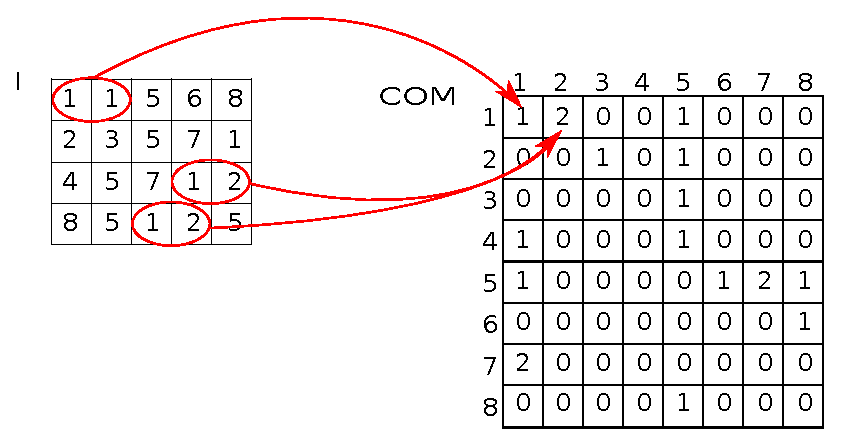
\includegraphics[scale=0.8]{GLCM.eps}
%  \caption{Example how the values in the GLCM are calclulated of the 4-by-5 image I. Element (1, 1) in the GLCM contains the value 1 because there is only one instance inf the image where two horizontally adjacent pixels have the values 1 and 1.}\label{GLCM}
%\end{figure}

Extending this method to three-dimensions it is necessary to look on how the offsets are defined because the size of the GLCM is defined by the amount of GIs and not by the images it is derived from. Considering a 3 $\times$ 3 $\times$ 3 matrix we have a possible of 26 offsets. In two-dimensions it is possible to eliminate half of the offsets because of the relation GLCM$_{d,d}^\textbf{T}$ = GLCM$_{-d,-d}$, and it is the same case in three-dimensions with the relation being GLCM$_{d,d,d}^\textbf{T}$ = GLCM$_{-d,-d,-d}$. This leaves 13 offsets which are illustrated below.\\

\begin{figure}[H]
  \centering
  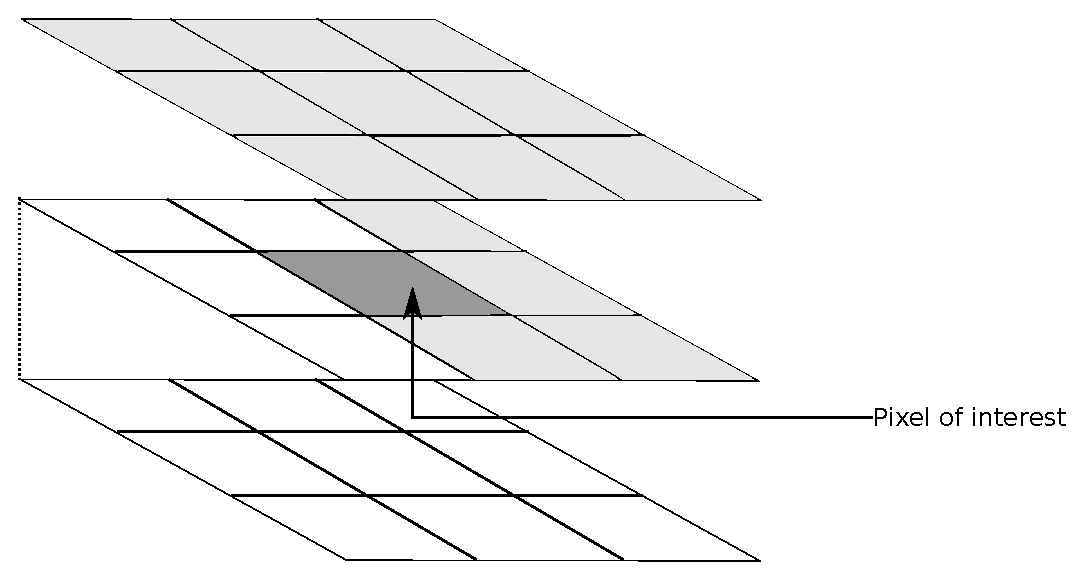
\includegraphics[scale=0.6]{3DCOM.eps}
  \caption{Example of the offsets for the 3D}\label{3DCOM}
\end{figure}



To create a two-dimensional GLCM on three-dimensional image we create slices through the image. Given a $n \times m \times l$, n = 20, m = 20 l = 20, image we can create a slice for each n. Slice$_1$ is equal to the matrix M( $n = 1 \times m \times l$), Slice$_2$ = M( $n = 2 \times m \times l$), and so on, giving a total of 20 $m \times l$ images instead. It is possible for each slice to calcualte the GLCM$_{d,d}$ for each slice, and we define GLCM$_{d,d}$ = $ \Sigma_{n=1}^20$ GLCM$_{d,d}$(Slice$_n$)

These slices are done in all three directions of the image for the four difference offsets resulting in 12 GLCMs. There is an overlap between six of the GLCMs. Slicing through n axis with offset (0,d) is equal to slicing through the m axis with the same offset. Slicing through the m axis with offset (-d,d) is equal to slicing through the l axis with offset (-d,0). Slicing through the l axis with offset (-d,d) is equal to slicing through the n axis with offset (d,0), which is the transposed offset of (-d,0). Removing the duplicates leaves nine GLCMs which we calculate at distances d = (1,2,...,10), giving a total of 90 GLCMs for each mri scan.

The three-dimensional versions is also calculated for distances d = (1,2,...,10) resulting in 130 GLCMs for each mri scan.

\subsection{Texture features from co-occurrence matrix}
To compare the differences between the GLCMS 13 different features are computed. They are the same as used in \cite{MRfreeborough} except for one difference. The difference is how the correlation is calculated as $\sum_{i,j} \frac{(i-\mu_i)(j-\mu_j)glcm(i,j)}{(\sigma_i \cdot \sigma_j)}$, where $\mu_i$, $\mu_j$, $\sigma_i$, $\sigma_j$ are the means and standard deviations of $C_i$ and $C_j$ respectively. This correlation is called the Pearson product moment correlation coefficient and it determines how correlated a pixel is to its neighbour, over the whole image\cite{graycoprops}\cite{Pearson}. We calculate two versions of these features, one where we normalized the COMs and one where we do not.


\section{Machine learning}

Machine learning is a method used to create complex models and algorithms that lend themselves to prediction, when the models are exposed to new data that should be able to teach themselves to grow and change.
There are several different categories of machine learning, one of them being supervised learning. In supervised laerning given a large sample of input and output pairings, the goal is to find the complex function that maps that relation between input and output. With a sufficient large dataset it would be possible to train a supervised algorithm to predict output values for some new input values that it have not seen before.


\subsection{10-fold cross-validation}
Given a model with unknown paramers and a training set to which the model can be fit then the fitting process optimizes the models parameters to fit the training data. Validating this model against independent data (test data) from the same data pool as the training, it will generally turn out that the model does not fit the test data as well as the training data. It is known as overfitting and is a problem when the size of the training data set is small. Cross-validation is used to counteract overfitting.

Dividing the entire data set into 10 groups at random, one subsample is saved for testing and the reamining nine is used to fit the model. The procedures is done so all subsamples get to be used to validate exactly one time and the validation result can then be averaged to produce a single estimation. This solves the problem of overfitting, as the validation data set is never used in to fit the model.
\fxnote[inline]{how does this remove overfitting?}

\subsection{Feature selection}
Feature selection is the process of selection af subset of relevant features for use in model contruction.
The main goal of feature selection is to choose a subset of the entire set of input features so the subset can predict the output with an accuracy comparable to using the entire set to predict the output, but with a large reduction in the computational cost.
When a dataset contains many feautres that are either redundant og irrelevant it is possible to remove them without incurring much loss of information. Features may be redundant due to the pressence of another feature with which it is strongly correlated, while they may be very informative for the model their information have already been provided by a different feature. Only choosing a subset of the possible features have the added advantage of decreasing the complexity of the model.

Sequential forward feature selection(SFS) is a greedy algorrithm to choose features.
It starts off with finding the best possible single feature to describe the model. Given the feature set of that single feature, the next step is to find which other feature would improve the predictiveness of the model and then add that to the set of selected featuers. It continues to grow the set of selected features, until the goal have been reached. The goal can either be a specific amount of features, a specific accuracy for the model or it can stop if all choices of a new feature would decrease the accuracy.
A problem with SFS is due to its greedy nature, there is no guarantee that the first feature selected is part of the optimal solution. Given three features X$_1$, X$_2$ and X$_3$ where X$_1$ is the best single feature, X$_2$ is second best and X$_3$ the worst, it does not necessitate that pairing {X$_1$, X$_2$ } is better than {X$_2$, X$_3$}, nor does it secure any other relation, meaning that the SFS does not guarantee the optimal solution. Which leads to one of the drawbacks of this feature selection, if a feature is selected it is not possible to exclude it later even if it would increase the evaluation score to do so.

\begin{lstlisting}[mathescape=true]
The algorithm for SFS with 10-fold cross validation
Step 1:
Set selected features Y = \emptyset
X = entire featuerset
Seperate dataset into 10 folds of equal size with 5 of each class, {K$_1$,K$_2$,...,K$_10$}.

Step 2:
For feature i= 1 to No. of features
	for fold j=1 to No. of folds
		Train a k-nn model on {Y,X$_i$} using fold K$_{1,2,...,10} \setminus $  K$_{j} $ as training
		Calcualte missclassification error of model on K$_j$
Average the error for all 10 folds.

Step 3:
F = feature with lowest error
X = X $\setminus$ F
Y = Y $\cup$ F

Step 4:
Continue step 2-3 until the missclassification error worsen or 15 features have been selected.
\end{lstlisting}
The algorithm is run on 10 different k values for the k-nn model, k = 1,2,...,10.

\subsubsection{Naive}

\subsection{K Nearest Neighbors algorithm}

The K Nearest Neighbor (KNN) is a methoed that is used for classification and regression. It should be noted, that KNN is a non parametric lazy learning algorithm, which means that it does note make any assumptions on the underlying data distribution. In other words, it means that the training phase is fast and KNN keeps all the training data. It should be noted that KNN makes decision based on the entire training data set and in the KNN an object is classified by majority vote of its neighbors, with the object being assigned to the class most common amongst its \textit{KNN}'s. \ref{fig:KNNK5}\\
Since the training phase is minimal, then it should be noted that the testing phase is very costly for KNN in both memory and time and often it can be a worst case for time needed, since all points might take point in the decision making.

\begin{figure}[H]
  \centering
  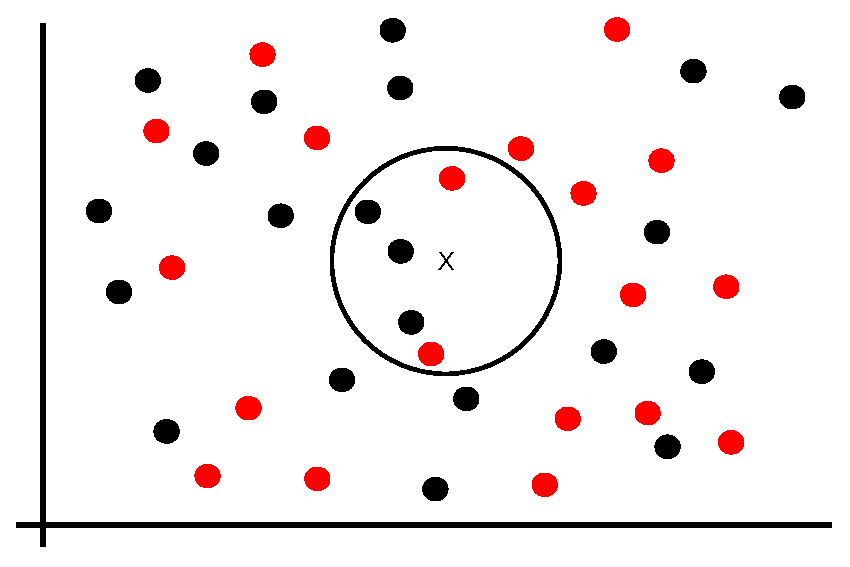
\includegraphics[scale=0.6]{KNNK5.eps}
  \caption{The KNN grows a spherical region until it encloses \textit{k} training samples, and labels the test point by a majority vote of these samples. In this \textit{k} = 5 case, the test point \textbf{x} would be labelled the category of the black points}\label{fig:KNNK5}
\end{figure}

Because the KNN classifer predicts the class of a given test observation by identifying the observations that are nearest to it, the scale of the variables matters. Image that we have a large scale variabels, they will have a much larger effect on the distance between observations and hence the KNN classifier, than variables on a small scale. Often a good way to handle this problem is to standardize the data.

The disadvantage of KNN is that choosing a \textit{k} may be tricky, so we are left to test the algorithm on multiple \textit{k}'s and often it needs a large number of samples for better accuracy.

Typically will the KNN classifier be based on a distance, commonly it is based on the Euclidean distance between a test sample and the specified training samples. Let $x_i$ be an input sample with $p$ features $(x_{i1}, x_{i2},...,x_{ip})$, and $n$ be the total number of input samples $i=1,2,...,n$ and $p$ the total number of features $j=1,2,...,p$. The Euclidean distance between sample $x_i$ and $x_l$, $l=1,2,...,n$ is defined as $d(x_i,x_l) = \sqrt{(x_{i1}-x_{l1})^2+(x_{i2}-x_{l2})^2+...+(x_{ip}-x_{lp})^2}$

\section{Erode}

Each patients hippocampus has been segmented in the MRI scan. The problems we can run into are that the background will blur with the segmentation i.e. the hippocampus. Performing a erosion can solve this problem and we can focus on the hippocampus, with the maximum number of details. As seen in figure \ref{fig:noterodeslice} the erosion has not been performed yet, but we might have some problems with data surrounding the hippocampus is blurring out the edges of the hippocampus. To solve this, we create a mask to separate the hippocampus from the background data and end up with what is left in figure \ref{fig:erodeslice}

\begin{figure}[H]
    \begin{subfigure}{.5\textwidth}
      \centering
      \includegraphics[scale=0.4]{noterodeSlice10x.eps}
      \caption{Note eroded}\label{fig:noterodeslice}
    \end{subfigure}
    \begin{subfigure}{.5\textwidth}
      \centering
      \includegraphics[scale=0.4]{erodeSlice10x.eps}
      \caption{After erosion has been performed}\label{fig:erodeslice}
    \end{subfigure}
    \caption{Hippocampus at slice 10 on the X-axis as bitwise}
\end{figure}

The erosion we have used is called a city-block metric and can be seen in figure \ref{fig:Erosion2D}.

\begin{figure}[H]
  \centering
    \begin{tikzpicture}[scale=0.5]
    \matrix[square matrix]
    {
    |[fill=white]| & |[fill=white]|   & |[fill=white]|   & |[fill=white]|   & |[fill=white]|\\
    |[fill=white]| & |[fill=white]|   & |[fill=red!30]|$N_2$ & |[fill=white]|   & |[fill=white]|\\
    |[fill=white]| & |[fill=red!30]|$N_1$ & |[fill=red!30]|$\boxplus$ & |[fill=red!30]|$N_3$ & |[fill=white]|\\
    |[fill=white]| & |[fill=white]|   & |[fill=red!30]|$N_4$ & |[fill=white]|   & |[fill=white]|\\
    |[fill=white]| & |[fill=white]|   & |[fill=white]|   & |[fill=white]|   & |[fill=white]| \\
    };
    \end{tikzpicture}
  \caption{Text}\label{fig:Erosion2D}
\end{figure}
To give an example of how the erosion works, it will be illustrated and we will use the city-block metric for this purpose. So we will use figure \ref{fig:Erosion2D} and erode the image in figure \ref{fig:ErosionExample}.
\begin{figure}[H]
  \begin{subfigure}{.3\textwidth}
    \centering
    \begin{tikzpicture}
    \matrix[square matrixlarge]
    {
    |[fill=white]| & |[fill=white]| & |[fill=white]| & |[fill=white]| & |[fill=white]| & |[fill=white]| & |[fill=white]| & |[fill=white]| & |[fill=white]| & |[fill=white]| \\
    |[fill=white]| & |[fill=white]| & |[fill=white]| & |[fill=white]| & |[fill=white]| & |[fill=white]| & |[fill=white]| & |[fill=white]| & |[fill=white]| & |[fill=white]| \\
    |[fill=white]| & |[fill=white]| & |[fill=white]| & |[fill=blue!30]| & |[fill=blue!30]| & |[fill=white]| & |[fill=white]| & |[fill=white]| & |[fill=white]| & |[fill=white]| \\
    |[fill=white]| & |[fill=white]| & |[fill=blue!30]| & |[fill=blue!30]| & |[fill=blue!30]| & |[fill=blue!30]| & |[fill=white]| & |[fill=white]| & |[fill=white]| & |[fill=white]| \\
    |[fill=white]| & |[fill=white]| & |[fill=blue!30]| & |[fill=blue!30]| & |[fill=blue!30]| & |[fill=blue!30]| & |[fill=white]| & |[fill=white]| & |[fill=white]| & |[fill=white]| \\
    |[fill=white]| & |[fill=white]| & |[fill=white]| & |[fill=blue!30]| & |[fill=blue!30]| & |[fill=blue!30]| & |[fill=blue!30]| & |[fill=white]| & |[fill=white]| & |[fill=white]| \\
    |[fill=white]| & |[fill=white]| & |[fill=white]| & |[fill=blue!30]| & |[fill=blue!30]| & |[fill=blue!30]| & |[fill=blue!30]| & |[fill=white]| & |[fill=white]| & |[fill=white]| \\
    |[fill=white]| & |[fill=white]| & |[fill=white]| & |[fill=white]| & |[fill=white]| & |[fill=blue!30]| & |[fill=white]| & |[fill=white]| & |[fill=white]| & |[fill=white]| \\
    |[fill=white]| & |[fill=white]| & |[fill=white]| & |[fill=white]| & |[fill=white]| & |[fill=white]| & |[fill=white]| & |[fill=white]| & |[fill=white]| & |[fill=white]| \\
    |[fill=white]| & |[fill=white]| & |[fill=white]| & |[fill=white]| & |[fill=white]| & |[fill=white]| & |[fill=white]| & |[fill=white]| & |[fill=white]| & |[fill=white]| \\
    };
    \end{tikzpicture}
    \caption{Original image}
    \end{subfigure}
    \begin{subfigure}{.3\textwidth}
    \begin{tikzpicture}
    \matrix[square matrixlarge]
    {
    |[fill=white]| & |[fill=white]| & |[fill=white]| & |[fill=white]| & |[fill=white]| & |[fill=white]| & |[fill=white]| & |[fill=white]| & |[fill=white]| & |[fill=white]| \\
    |[fill=white]| & |[fill=white]| & |[fill=white]| & |[fill=white]| & |[fill=white]| & |[fill=white]| & |[fill=white]| & |[fill=white]| & |[fill=white]| & |[fill=white]| \\
    |[fill=white]| & |[fill=white]| & |[fill=white]| & |[fill=red!50]| & |[fill=red!50]| & |[fill=white]| & |[fill=white]| & |[fill=white]| & |[fill=white]| & |[fill=white]| \\
    |[fill=white]| & |[fill=white]| & |[fill=red!50]| & |[fill=blue!30]| & |[fill=blue!30]| & |[fill=red!50]| & |[fill=white]| & |[fill=white]| & |[fill=white]| & |[fill=white]| \\
    |[fill=white]| & |[fill=white]| & |[fill=red!50]| & |[fill=blue!30]| & |[fill=blue!30]| & |[fill=red!50]| & |[fill=white]| & |[fill=white]| & |[fill=white]| & |[fill=white]| \\
    |[fill=white]| & |[fill=white]| & |[fill=white]| & |[fill=red!50]| & |[fill=blue!30]| & |[fill=blue!30]| & |[fill=red!50]| & |[fill=white]| & |[fill=white]| & |[fill=white]| \\
    |[fill=white]| & |[fill=white]| & |[fill=white]| & |[fill=red!50]| & |[fill=red!50]| & |[fill=blue!30]| & |[fill=red!50]| & |[fill=white]| & |[fill=white]| & |[fill=white]| \\
    |[fill=white]| & |[fill=white]| & |[fill=white]| & |[fill=white]| & |[fill=white]| & |[fill=red!50]| & |[fill=white]| & |[fill=white]| & |[fill=white]| & |[fill=white]| \\
    |[fill=white]| & |[fill=white]| & |[fill=white]| & |[fill=white]| & |[fill=white]| & |[fill=white]| & |[fill=white]| & |[fill=white]| & |[fill=white]| & |[fill=white]| \\
    |[fill=white]| & |[fill=white]| & |[fill=white]| & |[fill=white]| & |[fill=white]| & |[fill=white]| & |[fill=white]| & |[fill=white]| & |[fill=white]| & |[fill=white]| \\
    };
    \end{tikzpicture}
    \caption{Performing erode on the image}
    \end{subfigure}
    \begin{subfigure}{.3\textwidth}
    \begin{tikzpicture}
    \matrix[square matrixlarge]
    {
    |[fill=white]| & |[fill=white]| & |[fill=white]| & |[fill=white]| & |[fill=white]| & |[fill=white]| & |[fill=white]| & |[fill=white]| & |[fill=white]| & |[fill=white]| \\
    |[fill=white]| & |[fill=white]| & |[fill=white]| & |[fill=white]| & |[fill=white]| & |[fill=white]| & |[fill=white]| & |[fill=white]| & |[fill=white]| & |[fill=white]| \\
    |[fill=white]| & |[fill=white]| & |[fill=white]| & |[fill=white]| & |[fill=white]| & |[fill=white]| & |[fill=white]| & |[fill=white]| & |[fill=white]| & |[fill=white]| \\
    |[fill=white]| & |[fill=white]| & |[fill=white]| & |[fill=blue!30]| & |[fill=blue!30]| & |[fill=white]| & |[fill=white]| & |[fill=white]| & |[fill=white]| & |[fill=white]| \\
    |[fill=white]| & |[fill=white]| & |[fill=white]| & |[fill=blue!30]| & |[fill=blue!30]| & |[fill=white]| & |[fill=white]| & |[fill=white]| & |[fill=white]| & |[fill=white]| \\
    |[fill=white]| & |[fill=white]| & |[fill=white]| & |[fill=white]| & |[fill=blue!30]| & |[fill=blue!30]| & |[fill=white]| & |[fill=white]| & |[fill=white]| & |[fill=white]| \\
    |[fill=white]| & |[fill=white]| & |[fill=white]| & |[fill=white]| & |[fill=white]| & |[fill=blue!30]| & |[fill=white]| & |[fill=white]| & |[fill=white]| & |[fill=white]| \\
    |[fill=white]| & |[fill=white]| & |[fill=white]| & |[fill=white]| & |[fill=white]| & |[fill=white]| & |[fill=white]| & |[fill=white]| & |[fill=white]| & |[fill=white]| \\
    |[fill=white]| & |[fill=white]| & |[fill=white]| & |[fill=white]| & |[fill=white]| & |[fill=white]| & |[fill=white]| & |[fill=white]| & |[fill=white]| & |[fill=white]| \\
    |[fill=white]| & |[fill=white]| & |[fill=white]| & |[fill=white]| & |[fill=white]| & |[fill=white]| & |[fill=white]| & |[fill=white]| & |[fill=white]| & |[fill=white]| \\
    };
    \end{tikzpicture}
    \caption{The image after erosion}
    \end{subfigure}
  \caption{Example of a city-block erosion with before and after}\label{fig:ErosionExample}
\end{figure}

As seen in figure \ref{fig:ErosionExample} the noise (background) have been removed. This is an example in 2D. Now we wish to extend the erosion city-block to 3D. As seen in figure \ref{fig:Erosion2D} it have 4 neighbours and when we extend this to 3D we will end up with 6 neighbours instead as seen in figure \ref{fig:Erosion3D} and the concept is still the same as in 2D

\begin{figure}[H]
  \centering
    \begin{subfigure}{.3\textwidth}
    \centering
    \begin{tikzpicture}
    \matrix[square matrix]
    {
    |[fill=white]| & |[fill=white]|   & |[fill=white]|   & |[fill=white]|   & |[fill=white]|\\
    |[fill=white]| & |[fill=white]|   & |[fill=white]| & |[fill=white]|   & |[fill=white]|\\
    |[fill=white]| & |[fill=white]| & |[fill=red!30]|$N_5$ & |[fill=white]| & |[fill=white]|\\
    |[fill=white]| & |[fill=white]|   & |[fill=white]| & |[fill=white]|   & |[fill=white]|\\
    |[fill=white]| & |[fill=white]|   & |[fill=white]|   & |[fill=white]|   & |[fill=white]| \\
    };
    \end{tikzpicture}
    \caption{From above}
    \end{subfigure}
    \begin{subfigure}{.3\textwidth}
    \centering
    \begin{tikzpicture}
    \matrix[square matrix]
    {
    |[fill=white]| & |[fill=white]|   & |[fill=white]|   & |[fill=white]|   & |[fill=white]|\\
    |[fill=white]| & |[fill=white]|   & |[fill=red!30]|$N_2$ & |[fill=white]|   & |[fill=white]|\\
    |[fill=white]| & |[fill=red!30]|$N_1$ & |[fill=red!30]|$\boxplus$ & |[fill=red!30]|$N_3$ & |[fill=white]|\\
    |[fill=white]| & |[fill=white]|   & |[fill=red!30]|$N_4$ & |[fill=white]|   & |[fill=white]|\\
    |[fill=white]| & |[fill=white]|   & |[fill=white]|   & |[fill=white]|   & |[fill=white]| \\
    };
    \end{tikzpicture}
    \caption{From the front}
    \end{subfigure}
    \begin{subfigure}{.3\textwidth}
    \centering
    \begin{tikzpicture}
    \matrix[square matrix]
    {
    |[fill=white]| & |[fill=white]|   & |[fill=white]|   & |[fill=white]|   & |[fill=white]|\\
    |[fill=white]| & |[fill=white]|   & |[fill=white]| & |[fill=white]|   & |[fill=white]|\\
    |[fill=white]| & |[fill=white]| & |[fill=red!30]|$N_6$ & |[fill=white]| & |[fill=white]|\\
    |[fill=white]| & |[fill=white]|   & |[fill=white]| & |[fill=white]|   & |[fill=white]|\\
    |[fill=white]| & |[fill=white]|   & |[fill=white]|   & |[fill=white]|   & |[fill=white]| \\
    };
    \end{tikzpicture}
    \caption{From below}
    \end{subfigure}
  \caption{2D example of the 3D city-block}\label{fig:Erosion3D}
\end{figure}




